\section{Overview of the Universal Verification Methodology}\label{uvm}

The \emph{Universal Verification Methodology (UVM)} describes the Methodology to verify \emph{integrated circuit (IC)} designs. 
It is standardized by Accellera \cite{uvm}, an independent standards organization. 
One of the key principles is to create reusable verification environments and thereby enabling efficient development.
This is accomplished by using \emph{Universal Verification Components (UVCs)}.

\subsection{Universal Verification Components}\label{uvc}

A UVM testbench is composed of reusable and configurable UVCs, each containing all functionalities to verify a single interface or module.
The structure of these components inside a UVM testbench is shown in figure \ref{fig:uvm_testbench}.

\begin{figure}[htb]
 \centering
 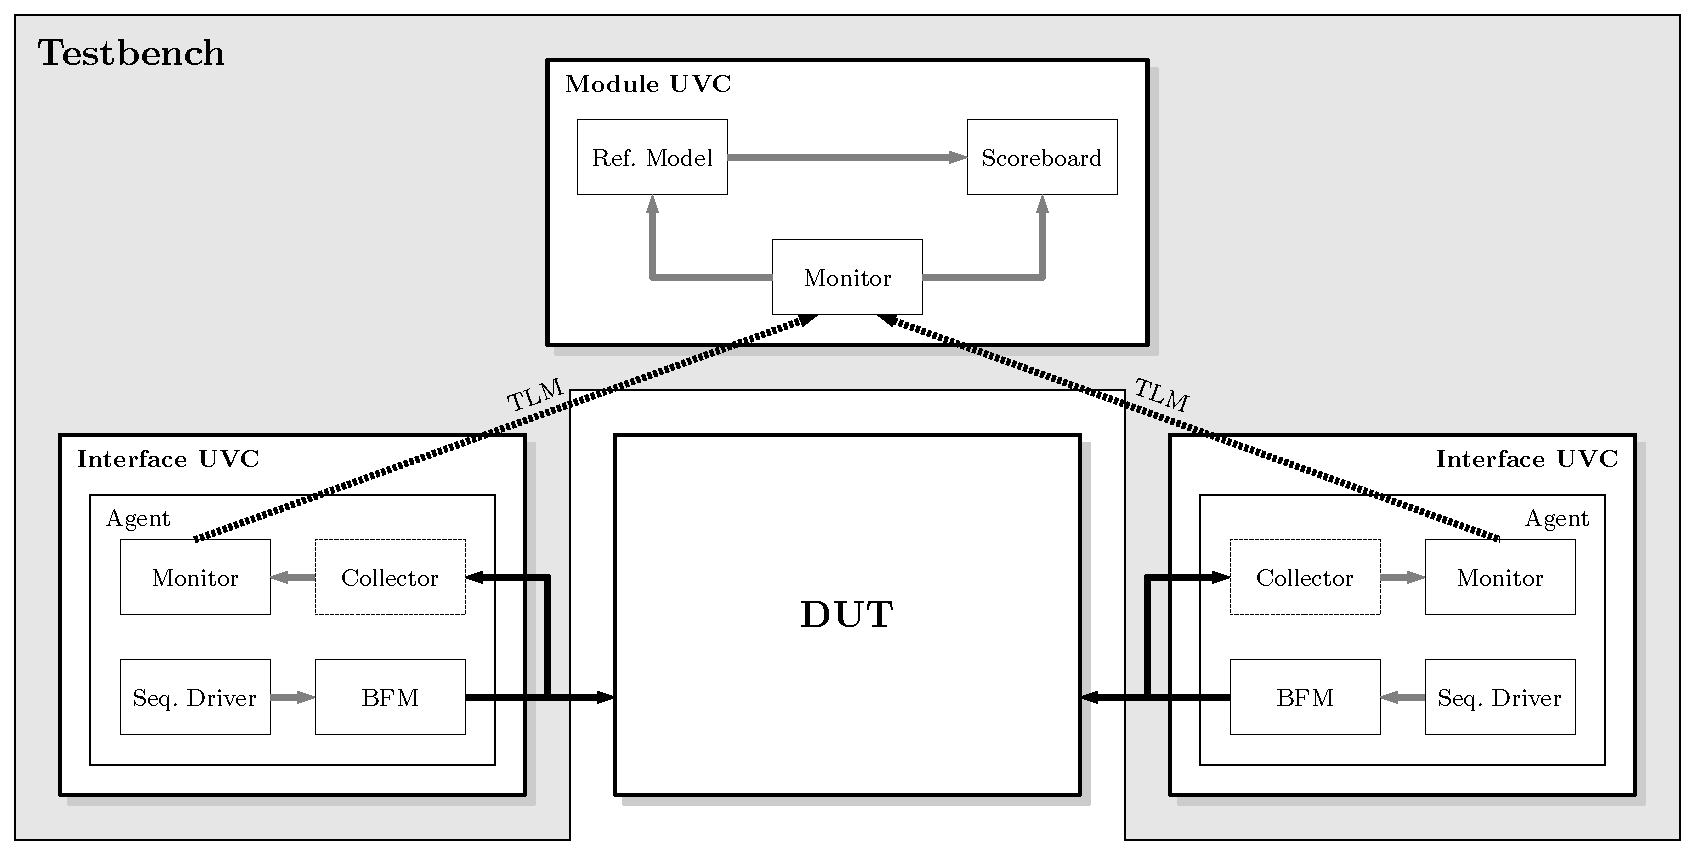
\includegraphics[width=1.0\textwidth,angle=0]{images/uvm_tb}
 %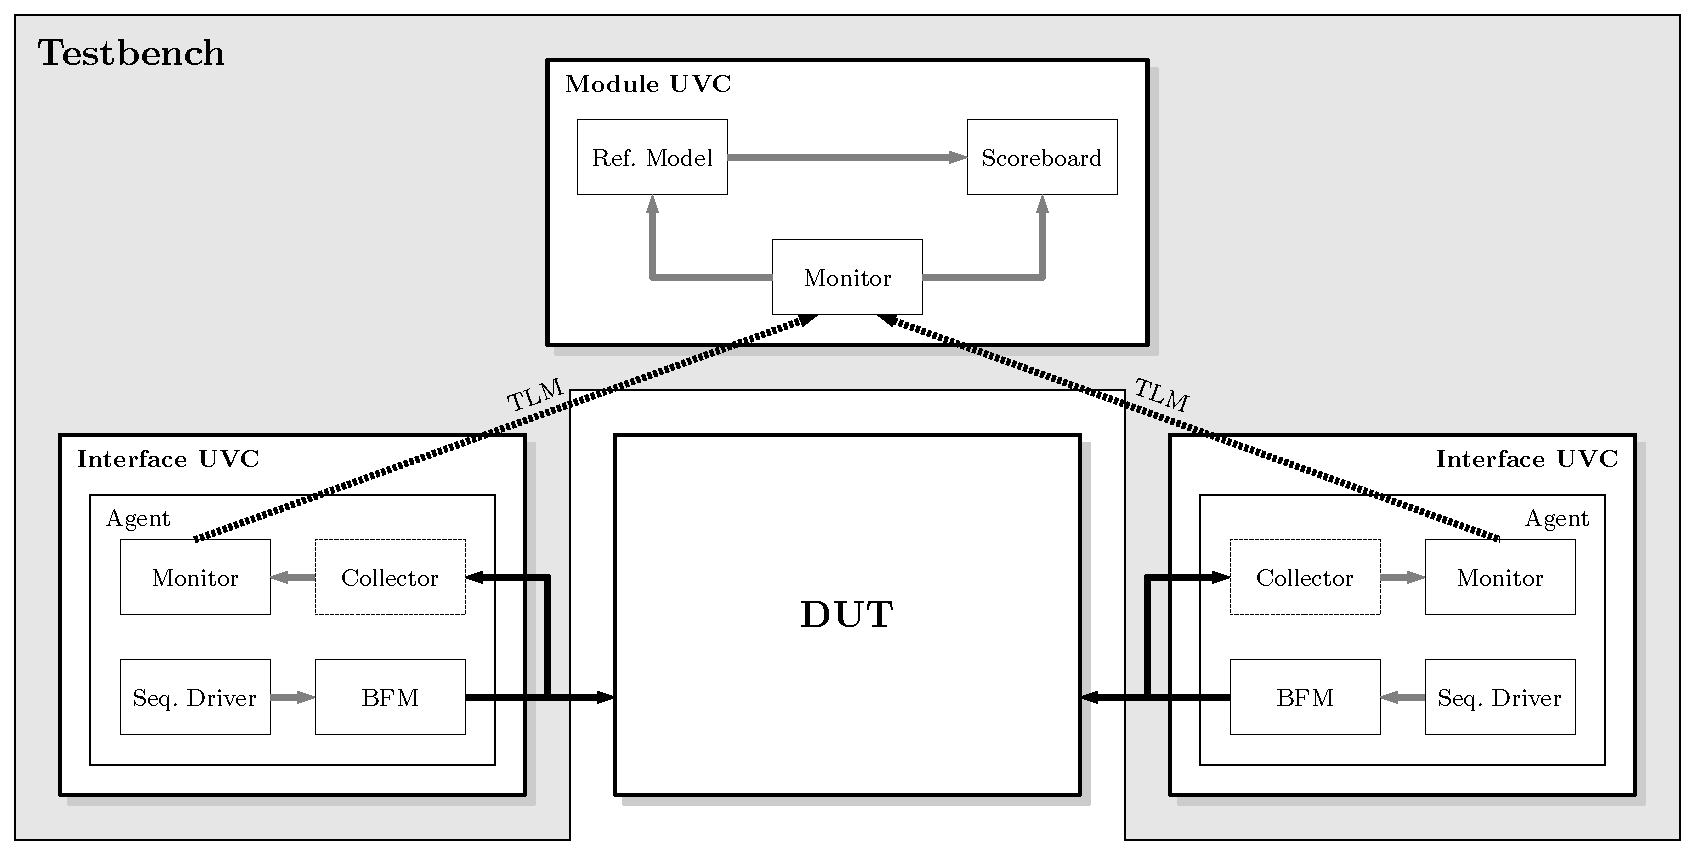
\includegraphics[scale=1.0]{images/uvm_tb}
 \caption{Structure of an UVM testbench}
\label{fig:uvm_testbench}
\end{figure}

\subsubsection{Interface UVC}\label{interface_uvc}

For each interface of an \emph{device under test (DUT)} an interface UVC has to be created. 
Its purpose is to establish the communication between the testbench and the signals of the DUT.
More than one interface UVC can be connected to the DUT. 
Its standard architecture contains the following elements \cite{uvm_sv}:

\begin{itemize}
  \item \textbf{Sequence item}\\
  Sequence items represent stimulus for an interface of the DUT or can be extracted from it for observation.
  The fields of a sequence item are derived from the attributes of the transaction.
  By this an object in a higher level of abstraction than the signals of the DUT themselves is created.
  \item \textbf{Sequence Driver}\\
  The active functionality of generating stimuli for an interface and driving it is split between two units.
  On the transaction-level, the sequence driver generates pseudo random stimuli.
  Therefore it executes sequences.
  These sequences contain other sequences or the above mentioned sequence items. 
  The sequence driver forwards sequence items to the bus functional model (BFM).
  \item \textbf{Bus Functional Model (BFM)}\\
  The BFM implements the signal-level unit of the stimuli generation process.
  It receives a sequence item from a sequence driver. 
  Then the attributes of the sequence item are used to drive the interface signals of the DUT.
  \item \textbf{Monitor}\\
  The monitor basically inverts the functionality of a BFM. 
  Where the BFM uses sequence items to drive an interface of the DUT, the monitor samples the signals of it.
  These data are then used to generate sequence items.
  Additionally it collects the coverage of the interface signals and performs checking on them.
  The monitor is a passive entity and does not drive any signals of the DUT.
  \item \textbf{Collector} (optional)\\
  Just like splitting stimuli generation into transaction-level and signal-level units the same can be done for the sampling process. 
  Thereby the monitor collects coverage and performs checking, but the signal-level functionality is transferred into another unit called collector.
  So the collector samples the interface signals and creates the corresponding sequence item.
  This partitioning is optional and not mandatory for UVM.
  \item \textbf{Agent}\\
  Agents encapsulate sequence drivers, BFMs and monitors to ensure re-usability.
  They can either be active and drive the signals of the DUT or passive and monitor the DUT's interface while other DUTs drive the signals.
  The active elements of an agent are the sequence driver as well as the BFM and passive ones are the collector and the monitor. 
  The passive elements of an UVC are also used when the agent is configured as active. 
  UVCs can contain more than one agent, for example master or slave agents.
  \item \textbf{Environment}\\
  The environment is the top-level entity of the UVC. 
  It encapsulates all its agents as well as configuration properties, which are used to customize the UVC and thereby increase its re-usability.
\end{itemize}

\subsubsection{Module UVC}\label{module_uvc}

Because an interface UVC can only capture information of a single interface, module UVCs are necessary to verify data across multiple interfaces. 
They are connected to interface UVCs via \emph{Transaction-Level Modeling (TLM) ports} (see section \ref{tlm}).\\
While verifying a DUT, more data is created than can be checked manually.
Therefore the testbench has to be self-checking.
A scoreboard and optionally a reference model are used for this purpose.

\paragraph{Scoreboard}
The scoreboard verifies the proper operation of the design by comparing the data driven into the DUT to the ones produced by it.
Depending on the design, the input data has to be processed, before it can be matched to the produced ones.
This can either be done in the scoreboard itself or for more complex operations in an additional unit called reference model.

\paragraph{Reference Model}
The reference model emulates the functionality of the DUT by predicting the expected result of the design for given input data.
Furthermore, it can provide information about the state of the DUT, which cannot be derived directly from the interfaces of the design.
These can then be used for checking, collecting coverage or generating new traffic.\\

There are three levels of precision for the implementation of a reference model \cite{cdnshelp}:

\begin{itemize}
  \item \textbf{Rough-Justification}\\
  Given the inputs and outputs of the DUT, the reference model can validate the behavior of the design.
  \item \textbf{Transaction-Level Functionality}\\
  Here the reference model predicts outputs of the design on transaction-level for given inputs.
  The results can then be used in the scoreboard to compare the actual outputs of the DUT to these predicted ones. 
  \item \textbf{Cycle-Accurate}\\
  A cycle-accurate reference model is the most precise one. 
  It also predicts the outputs of the DUT for given inputs like the transaction-level based.
  Additionally to functionally predicting the outputs, it emulates them cycle-accurate.
  This can be used for cycle-accurate stand-in mode.
  In this mode the testbench is executed without the DUT, which enables the development of the testbench prior to the design.\\
  This level is typically overkill, when the output is only used in the scoreboard.
\end{itemize}

\subsubsection{Data Communication between Components}\label{tlm}

To communicate between UVCs, TLM ports are used.
They provide the ability to exchange sequence items between components.
With TLM ports, the producing and consuming components can easily be swapped for alternative models, as long as they use the same TLM interface.
This improves re-usability of the UVCs \cite{uvm_sv}.

\subsection{Metric Driven Verification}

Test patterns can be used to test specific behaviors of the DUT \cite{uvm_e}. Thereby, each pattern handles a single scenario.
These patterns are manually created and require checking the behavior of the DUT by hand.
Since this kind of verification requires a lot of resources, other routes have to be chosen to reduce the costs of verification.\\
Using Metric Driven Verification (MDV) \cite{fv}, these hand-crafted specific test patterns are replaced with machine generated stimuli.
Thereby, the stimuli targets multiple scenarios instead of a single one.
With the automatically created stimuli, a larger amount of tests can be run.
Using MDV, the stimuli generation is embedded in the verification environment. Thereby, the driver can react to the state of the DUT and so improve the quality
of the stimuli.
The disadvantage of MDV is that the ability to ensure, that all interesting scenarios are verified, is reduced.
By collecting coverage, a measurement for the effectiveness of the verification is found.
Untested areas of the design can easily be identified.
The tests can then be modified to address these areas.
